% %%%%%%%%%%%%%%%%%%%%%%%%%%%%%%%%%%%%
% A LaTeX template for the technical essay of TTM4137 Wireless Security
% Stig F. Mjolsnes, 01.09.2012
%%%%%%%%%%%%%%%%%%%%%%%%%%%%%%%%%%%%%
\documentclass[a4paper,11pt]{article}

\usepackage[plain]{fullpage}
\usepackage{graphicx}  %This enables the inclusion of pdf graphic files in figures
\usepackage{hyperref} % Make links in your document click-able NB: must be loaded before the caption-package
\usepackage{caption}
\usepackage{subcaption}
\usepackage{wrapfig}
\usepackage[utf8]{inputenc}


\title{Attacks on Near Field Communications on Mobile Phones}
\author{Håkon Nymo Matland \\
	\texttt{hakonnym@stud.ntnu.no}\\
	TTM4137 Wireless Security Technical Essay}
\date{\today}

\begin{document}
\maketitle

\section{Introduction}
The Near Field Communication (NFC) technology is being deployed in mobile phones all over the world. The technology's applications is wide~\cite{remedios2006nfc}. Several companies focus on one of it's most promising applications: payment solutions using NFC~\cite{tan2013}. An analysis by Berg Insight claim that one in three mobile phones will come with NFC by 2017~\cite{nfc_growth}, making the technology a huge future marked.
The need of security and robustness is very important, as an insecure and attackable device would open criminals to steal funds, or simply take control over the device. Different attacks have been proven successful and malicious, and the threat should be taken seriously by both individuals and corporations. Simple RFID-stickers and vulnerabilities in software is all an attacker need to do harm. This essay will present and discuss some of the successful attacks previously demonstrated by experts in the field of NFC and security.


\section{Problem Discussion}

\subsection{Requirements of Form}

\begin{wrapfigure}[10]{r}{0.25\textwidth}
  \centering
  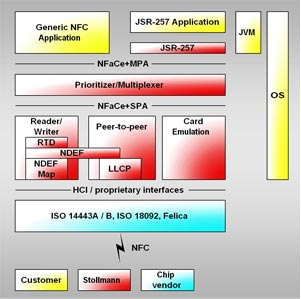
\includegraphics[scale=0.2]{nfc_stack} %Note: no use of .jpg file ending
  \vspace{-0.2cm}
  \caption{NFC stack}
  \label{fig:nfc_stack}
\end{wrapfigure}

We set the following requirements with respect to format:
\begin{enumerate}
	\item This \LaTeX\ template must be used.
	\item The whole document must be limited to~3~A4~pages (references not included).  A technical essay different from three -3- pages will be returned to the author
to be cut or enhanced to three pages.
	\item One or more illustrations in the form of figures, tables or diagrams must be included (see \hyperref[fig:nfc_stack]{Figure~\ref*{fig:nfc_stack}}).
	\item The entries in your \hyperref[sec:references]{reference} should be structured like follows:
	Author/Origin. \textit{Title}. Where, and when, published.
	\item The submitted file format must be pdf.
\end{enumerate}


\paragraph{Structure}  If you want  further substructure than sections and subsections, then you can use
a paragraph title like here.  This will look much better than introducing another numbered level of subsubsection.

\subsection{Requirements of Content}
 The text should be intelligible, logical, interesting and easy to read. Write for
your fellow engineering students, and assume that the reader has the same general theoretical
background as yourself. Use definitions, facts and logical argumentation. 

Interpret and refine the title, discuss the problem and intended scope in the
introduction. In the text, do not introduce facts that are not analysed later and
that are not relevant to your problem. Bring your \emph{own analysis and thinking} into
the essay. If you can, bring in new ideas. When you include tables or figures (see \hyperref[fig:linksys]{Figure~\ref*{fig:linksys}}), 
they should be referred to and explained in the text.

While it is allowed to cite Wikipedia or another web page, 
it is not recommended.
It is much better if you can refer to a technical article or paper.

\section{Conclusion}
The submitted technical essays will be graded and contribute 20\% to the final grade of the course. The two best essays will be honoured with publication at It's learning, edited if necessary and become part of this year's  syllabus.

\begin{figure}[hbp]
	\centering
	\begin{subfigure}[b]{0.3\textwidth}
		\centering
		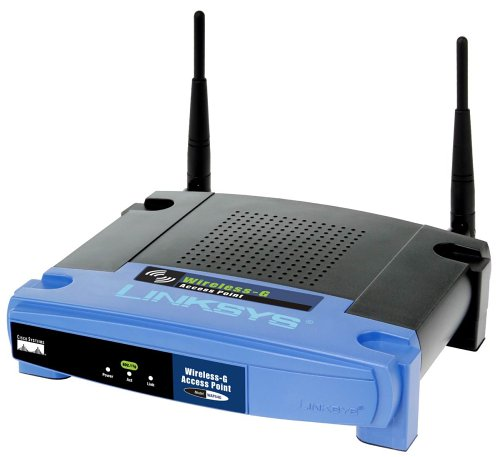
\includegraphics[scale=0.20]{linksys}
		\caption{Scale=0.20}
	\end{subfigure}
	\begin{subfigure}[b]{0.3\textwidth}
		\centering		
		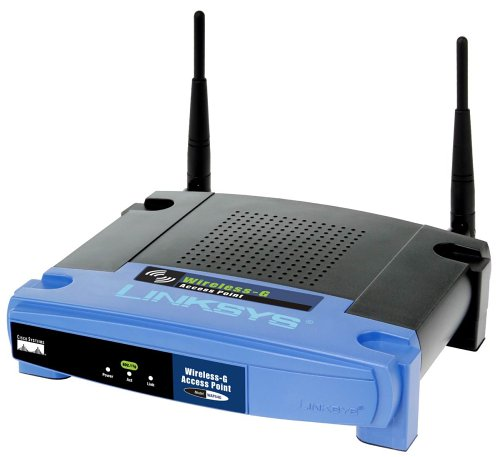
\includegraphics[scale=0.15]{linksys}
		\caption{Scale=0.15}	
	\end{subfigure}
	\begin{subfigure}[b]{0.3\textwidth}
		\centering		
		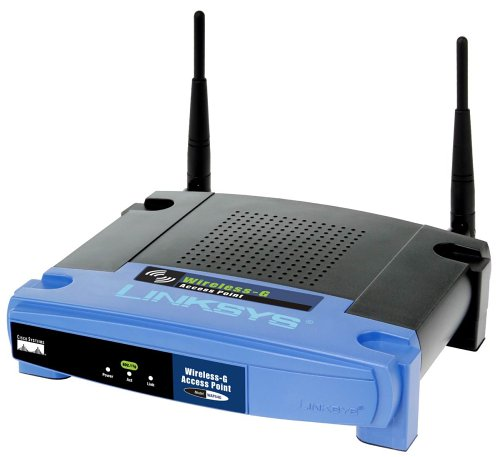
\includegraphics[scale=0.10]{linksys}
		\caption{Scale=0.10}
	\end{subfigure}
	\caption{The Linksys WRT54G line of routers include both  802.3 Ethernet and 802.11b/g wireless LAN.}
	\label{fig:linksys}
\end{figure}

% It is highly recommended to keep your references in a separate file (here called "references.bib")
% However if you want to create the reference section manually, 
% uncomment the lines below starting at "\begin{thebibliography} ... etc"
\bibliographystyle{unsrt}
\bibliography{references}\label{sec:references}



%\begin{thebibliography}{N}\label{sec:references}
%\bibitem{wiki1} Wikipedia. \textit{Citation.} Available at \url{http://en.wikipedia.org/wiki/Citation}.
%
%\bibitem{Daborn} Gordon Baxter, Jon Lewis and Ishbel Duncan. \textit{What is a Technical Essay?}
%Available online at \url{http://ishbel.host.cs.st-andrews.ac.uk/WhatisaTechnicalEssay.pdf}.
%
%\bibitem{Kortvedt} Henning Kortvedt and Stig Frode Mj{\o}lsnes. \textit{Eavesdropping Near Field Communication}.  
%In The Norwegian Information Security Conference (NISK 2009) Proceedings, pp. 57-68.  Tapir Akademiske Forlag, 2009.
%
%\end{thebibliography}  


\end{document} 
